\documentclass{beamer}
\usepackage{amsmath}
\usepackage{amssymb}
\usepackage{pgf}
\usepackage{tikz}
\usepackage{listings}
\usepackage{color}
\usepackage{nicefrac}
\usetikzlibrary{matrix}
\usetheme{boxes}
\newcommand{\fig}{./figures} % common figure path
\newcommand{\dbbslsh}{\textbackslash \textbackslash} % common figure path
\newenvironment{myblock}[3]{%
\definecolor{smtbx}{rgb}{0.64,0.76,0.68}
\setbeamercolor{block body}{#2}
\setbeamercolor{block title}{#3}
\begin{block}{#1}}{\end{block}}
\newcommand{\frnzplt}{FranzPlot }
\DeclareMathSymbol{\shortminus}{\mathbin}{AMSa}{"39}

\title[Curve e Sup. - Lab 3]{Curve e Superfici per il Design \\ Laboratorio - 4}
\author[Prof. Parolini]{Prof. Nicola Parolini}
%\institute[dimat]{Long Inst.}
\date{7 Novembre 2019}

\begin{document}

\begin{frame}
\maketitle
\end{frame}

\begin{frame}
\frametitle{Materiali}
Il materiale per l'esercitazione di oggi:
\begin{itemize}
\item Questa presentazione \\ (\texttt{Materiale Didattico/Laboratori/lab 4/lab4\_testo.pdf});
%\item Il file \texttt{es\_dado\_ref.toml} con l'esercizio risolto della passata esercitazione.
\item L'eseguibile del \frnzplt \\ (\texttt{Software/Franzplot 19.08 - Windows.exe})
\end{itemize}
\end{frame}


\section{Riepilogo}

\begin{frame}
\frametitle{Riepilogo}
    Per scrivere una retta in forma parametrica necessito di un \textbf{vettore direttore}
    e di un \textbf{punto appartente alla retta} (a volte chiamato \textit{termine noto}).

    \vspace{0.2cm}
    Sia $\mathbf v$ il vettore direttore e sia $\mathbf P$ il punto appartenente alla retta,
    allora la forma parametrica sar\`a $r(t) = \mathbf v t + \mathbf P$, con $t\in \mathbb{R}$.
    
    Scritto come sistema lineare:
\begin{displaymath}
    r(t) :\begin{cases} x = v_x t + P_x\\ y = v_y t + P_y \\z = v_z t + P_z \end{cases}
\quad t\in \mathbb{R}
\end{displaymath}

    \vspace{0.2cm}
    Il nome del parametro \`e arbitrario (tipicamente useremo $t$ o $s$).
    
    \`E sempre importante specificare l'intervallo di appartenenza.
\end{frame}

\begin{frame}
    \frametitle{Rette in \frnzplt}
    Per disegnare una qualsiasi curva parametrica in \frnzplt introduciamo i nodi \texttt{Geometries > Curve} e \texttt{Parameters > Interval}.

    \vspace{0.25cm}
    Il nodo \texttt{Interval} ci permette di definire il nome del parametro e l'intervallo cui appartiene.

    \vspace{0.25cm}
    Nel nodo \texttt{Curve} andiamo a inserire le coordinate $x$, $y$ e $z$ in funzione del parametro usato nel nodo \texttt{Interval}. Prendiamo ad esempio
    la seguente curva:

$$
r: \quad \left\{
\begin{array}{lcr}
x&=&3t+1\\
y&=&t-3\\
z&=&-2t
\end{array}
\right.
    \quad t\in \left[ \shortminus 10, 10 \right]
$$
    \end{frame}
    
\begin{frame}
    \frametitle{Rette in \frnzplt}
    Per visualizzare questa curva, creeremo il seguente grafo:
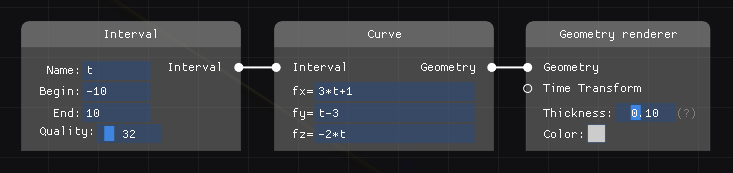
\includegraphics[width = 0.9\textwidth]{\fig/lab4_intro.png}
    L'output del nodo \texttt{Curve} \`e una Geometria, e come tale possiamo applicargli trasformazioni o animazioni.

    Una curva \`e una una Geometria 1D, possiamo usare lo slider \texttt{thickness} per modificare lo spessore usato nella visualizzazione.

    \vspace{0.5cm}
    Nota: nel nodo \texttt{Interval} non \`e possibile selezionare l'intero $\mathbb R$, quindi per \textbf{visualizzare} le rette scegliamo sempre un intervallo
    con valori sufficientemente grandi.

    \end{frame}

\section{Esercizi}
\begin{frame}
    \frametitle{Esercizio 1}

Date le seguenti rette nello spazio si calcoli, se esiste, il punto di intersezione:

$$
r:\left\{
\begin{array}{l}
x=3t+1\\
y=t-3\\
z= -2t
\end{array}
\right ., \qquad w:\left\{
\begin{array}{l}
x=s+3\\
y=4\\
z=-s+5
\end{array}
\right .
$$

    con $t, s \in \mathbb R$

    (Suggerimento: voglio che $r_x = w_x, \quad r_y = w_y, \quad r_z = w_z$)
    
    \vspace{1cm}
    Le rette sono perpendicolari?

    \end{frame}
    

\begin{frame}
\frametitle{Esercizio 2}

Siano assegnate le rette $r$ e $s$ di equazione
$$
r: \quad \left\{
\begin{array}{lcr}
x&=&3t-3\\
y&=&t-2\\
    z&=&-2t+4
\end{array}
\right. \qquad \qquad s: \quad \left\{
\begin{array}{lcr}
x&=&t\\
y&=&t-1\\
z&=&2t-2
\end{array}
\right.
$$

    \begin{itemize}
    \item $r$ ed $s$ sono perpendicolari? 
    \item Si visualizzino le rette $r$ e $s$ usando \frnzplt
    \end{itemize}
    
    \vspace{0.75cm}
    (Reminder: due rette sono perpendicolari se sono incidenti e le loro direzioni formano un angolo retto)
\end{frame}

\begin{frame}
\frametitle{Esercizio 3}
Dati i punti
$$
\mathbf{P}=\left[
\begin{array}{c}
0\\
-2\\
-1
\end{array}
\right]
\qquad
\mathbf{R}=\left[
\begin{array}{c}
3\\
-1\\
2
\end{array}
\right] \qquad
\mathbf{S}=\left[
\begin{array}{c}
-2\\
1\\
0
\end{array}
\right] 
$$
si calcolino:
    \begin{itemize}
    \item una rappresentazione parametrica della retta $r$ \\ passante per $\mathbf{P}$ e $\mathbf{R}$.
    \item una rappresentazione parametrica della retta $s$ \\ passante per $\mathbf{P}$ e $\mathbf{S}$.
    \end{itemize}
    
Le due rette sono perpendicolari?
\end{frame}

    
%
%
\begin{frame}
\frametitle{Esercizio 4}
\begin{itemize}
\item Rappresentare la retta $r$ passante per i punti
\begin{displaymath}
\mathbf{P}=\begin{bmatrix}2\\1\\1 \end{bmatrix},\;\;\;\;\;
\mathbf{Q}=\begin{bmatrix}1\\1\\3 \end{bmatrix};
\end{displaymath}
\item Determinare la retta $s$ perpendicolare ad $r$ e passante per:
\begin{displaymath}
\mathbf{M}=\begin{bmatrix}1\\2\\-2 \end{bmatrix}.
\end{displaymath}
\end{itemize}
\end{frame}


\end{document}
